\documentclass[10pt, a4paper]{letter}
\usepackage{advdate}
\usepackage{graphicx}
\usepackage[newdimens]{labels}
\usepackage{emerald}
\usepackage[scaled]{uarial}
\renewcommand*\familydefault{\sfdefault} %% Only if the base font of the document is to be sans serif
\usepackage[T1]{fontenc}
\usepackage{forloop}

\normalsize\sf
\LabelGridtrue
\LabelInfotrue

% MONTH NAMES
\newcommand{\MONTH}{%
  \ifcase\the\month
  \or Jan% 1
  \or Feby% 2
  \or Mar% 3
  \or Ap% 4
  \or May% 5
  \or Jun% 6
  \or Jul% 7
  \or Aug% 8
  \or Sep% 9
  \or Oct% 10
  \or Nov% 11
  \or Dec% 12
  \fi}

% HONEY LABELS
\LabelCols=2% Number of columns of labels per page
\LabelRows=6% Number of rows of labels per page

\LeftPageMargin=2mm% These four parameters give the
\RightPageMargin=5mm% page gutter sizes. The outer edges of
\TopPageMargin=1mm% the outer labels are the specified
\BottomPageMargin=5mm% distances from the edge of the paper.
\InterLabelColumn=10mm% Gap between columns of labels
\InterLabelRow=10mm% Gap between rows of labels
\LeftLabelBorder=10mm% These four parameters give the extra
\RightLabelBorder=10mm% space used around the text on each
\TopLabelBorder=10mm% actual label.
\BottomLabelBorder=10mm% actual label.

\begin{document}
\newcounter{ct}

\newcommand\honeylabel{%
{\fontsize{15.5pt}{20pt}\selectfont  \textbf{BAGBATCH\hfil MEADOW\hfil HONEY}} 
  \begin{tabular}{ll}%
    \begin{minipage}{2cm}%
      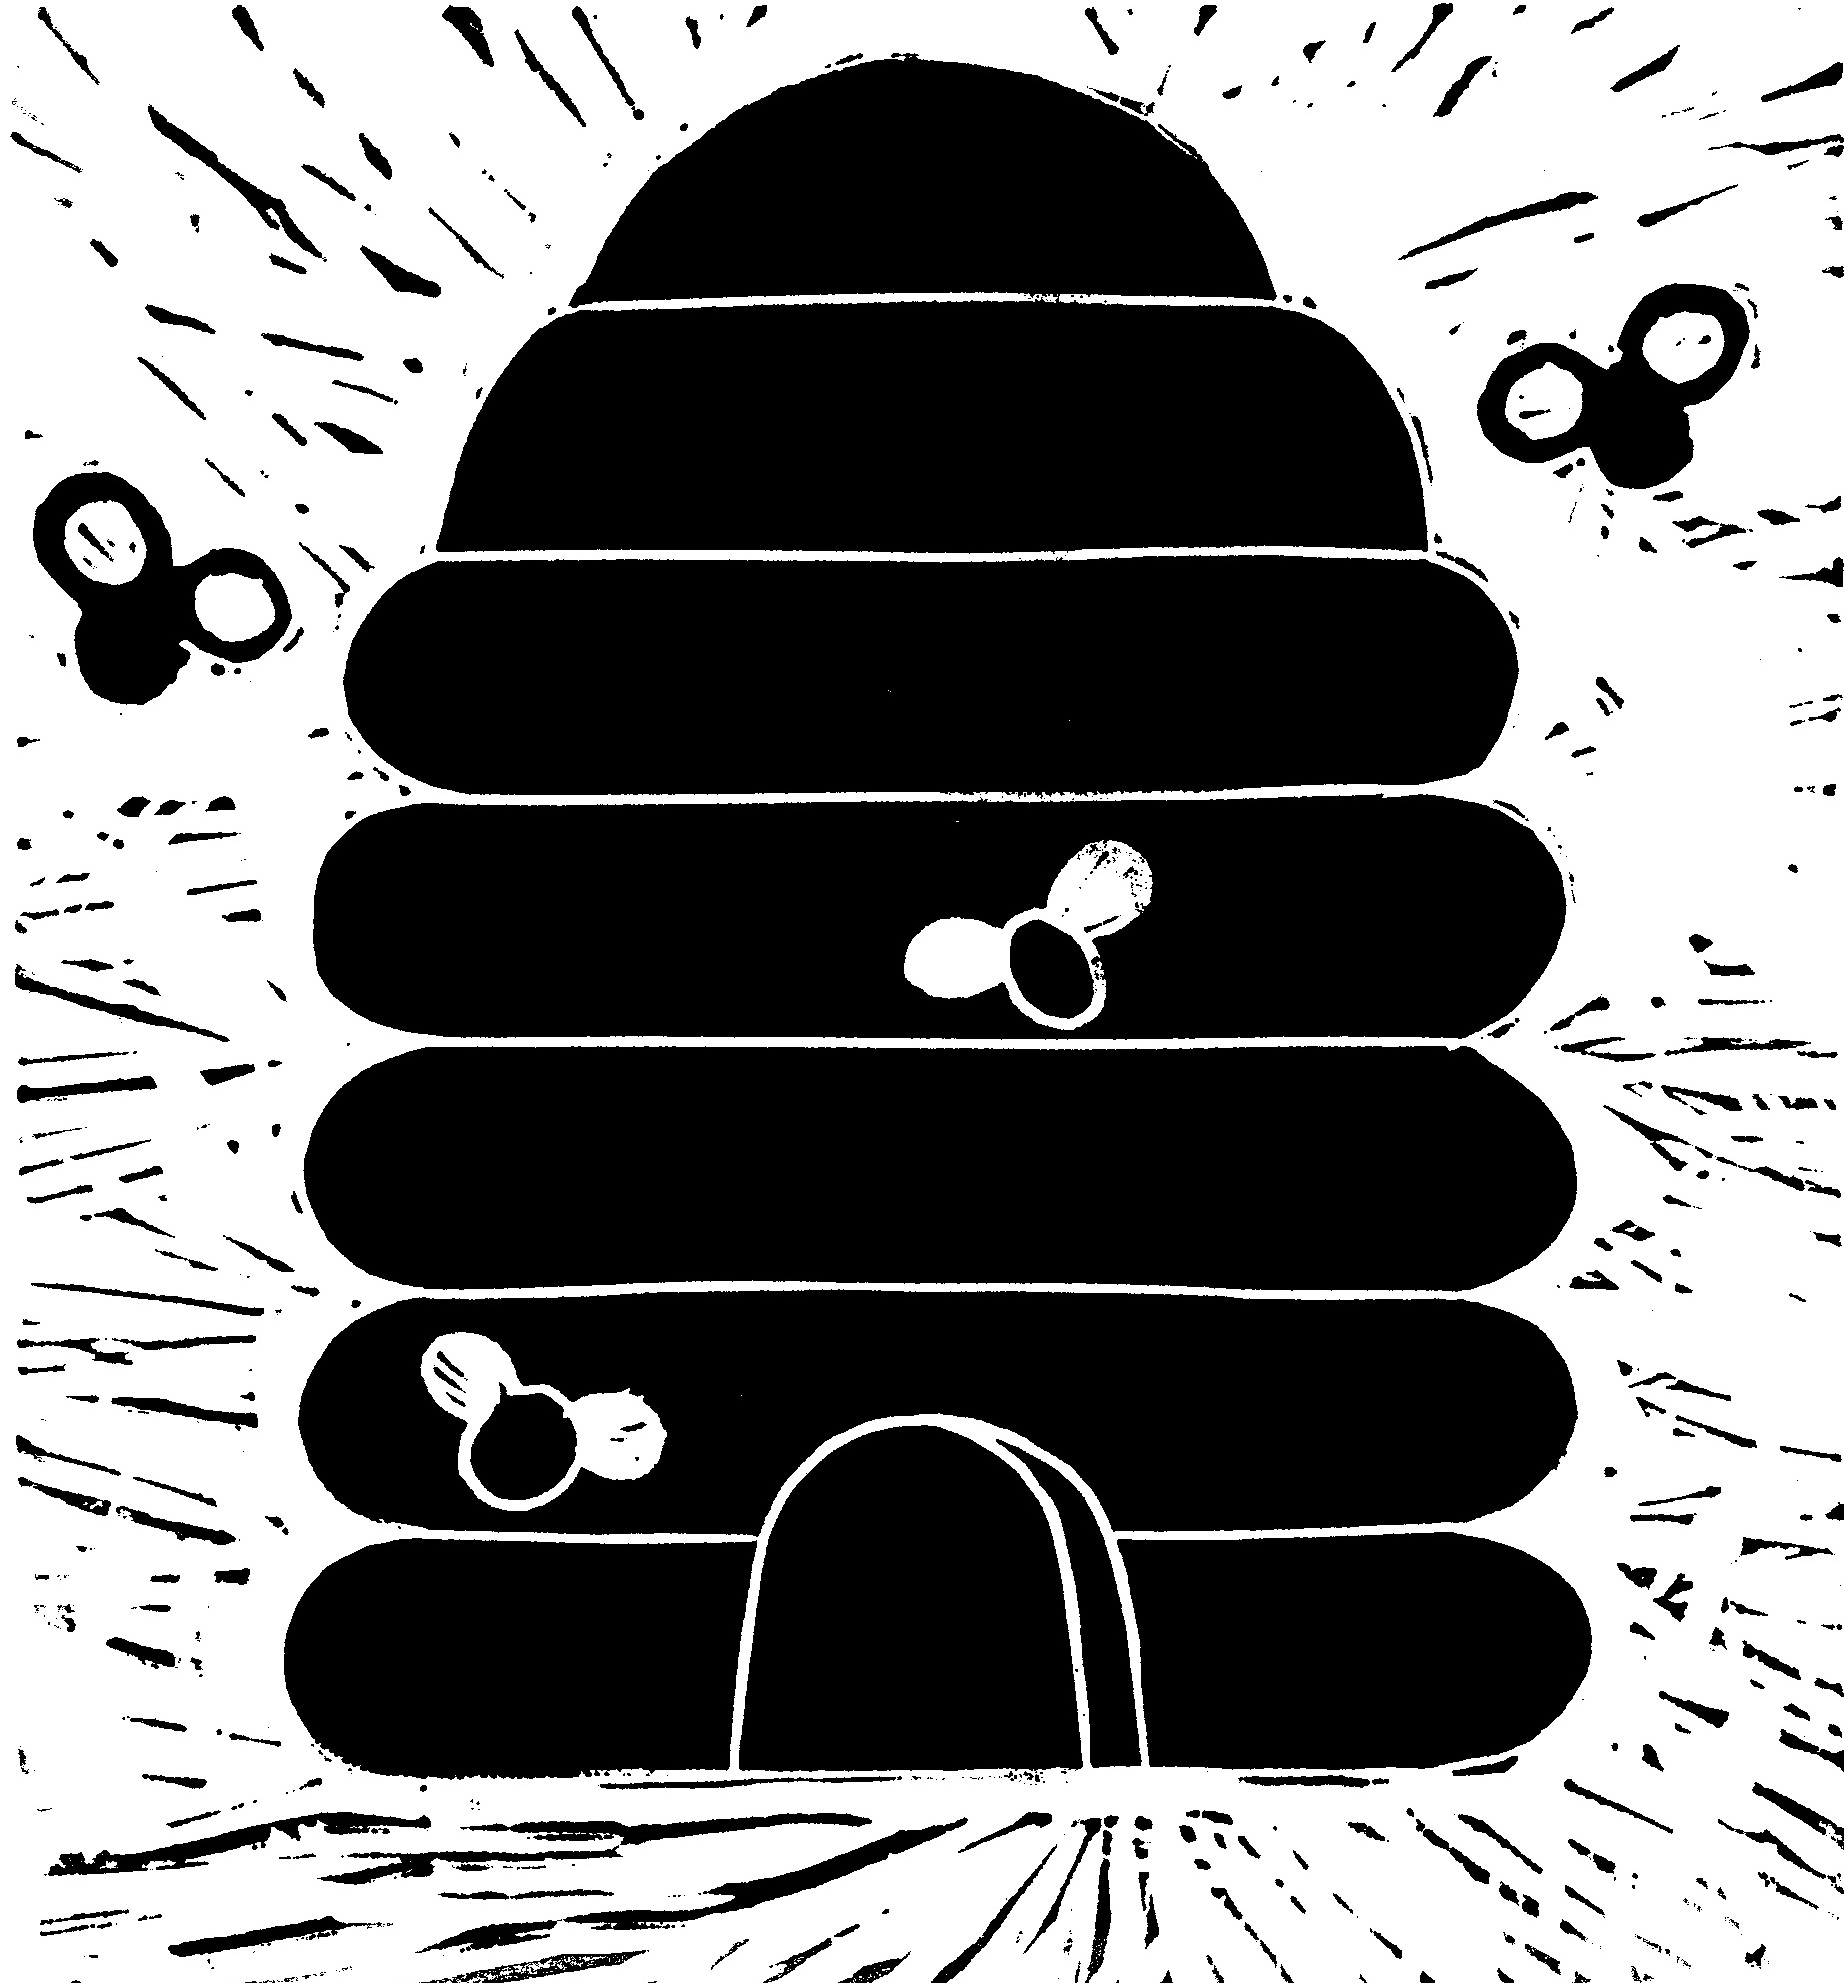
\includegraphics[width=2cm]{meadow-honey-skep-lino-cut.jpg}
    \end{minipage}%
    &
    \begin{minipage}{4.5cm}
     \par
      454g 1lb \hfill \ECFAugie Joe Collins\\
      \footnotesize\strut\hfill Bagbatch\\
      \strut\hfill All Stretton\\
      \strut\hfill  Shropshire\\
      Batch Beryl-\the\month \hfill SY6 6LA\\
      \AdvanceDate[730]% Add 3 years, 365 * 2 = 730
      Best before \MONTH-\the\year{} \hfill\strut 
    \end{minipage}
  \end{tabular}
{\fontsize{14pt}{20pt}\selectfont  \textbf{Harvested in Shropshire England}}
}% 

\begin{labels}
\forloop{ct}{0}{\value{ct} < 12}%
{%
  \honeylabel
  
}%
\end{labels}

% RAW LABELS
\LabelCols=3% Number of columns of labels per page
\LabelRows=7% Number of rows of labels per page
\LeftLabelBorder=5mm% These four parameters give the extra
\RightLabelBorder=5mm% space used around the text on each
\TopLabelBorder=5mm% actual label.
\BottomLabelBorder=5mm% actual label.
\LabelSetup%
\newcommand\rawlabel{%
  \small
  {\bf RAW HONEY} is the most original sweet liquid that honeybees produce from the concentrated nectar of flowers. 
   Collected straight from the honey extractor; it is totally unheated, unpasteurized, unprocessed honey.\vfill
}%

\begin{labels}
\forloop{ct}{0}{\value{ct} < 21}%
{%
  \rawlabel
  
}%
\end{labels}


% TAMPER STRIPS
\LeftPageMargin=0mm
\LabelSetup
\setlength{\parskip}{1em}
\forloop{ct}{0}{\value{ct} < 40}%
{%
  \rule{\paperwidth}{3pt}\par\par
}%

\end{document}

